\documentclass[12pt, a4paper, twopage]{scrartcl}
%\documentclass[
%11pt, % The default document font size, options: 10pt, 11pt, 12pt
%oneside, % Two side (alternating margins) for binding by default, uncomment to switch to one side
%chapterinoneline,% Have the chapter title next to the number in one single line
%english, % ngerman for German
%singlespacing, % Single line spacing, alternatives: onehalfspacing or doublespacing
%draft, % Uncomment to enable draft mode (no pictures, no links, overfull hboxes indicated)
%nolistspacing, % If the document is onehalfspacing or doublespacing, uncomment this to set spacing in lists to single
%liststotoc, % Uncomment to add the list of figures/tables/etc to the table of contents
%toctotoc, % Uncomment to add the main table of contents to the table of contents
%parskip, % Uncomment to add space between paragraphs
%nohyperref, % Uncomment to not load the hyperref package
%headsepline, % Uncomment to get a line under the header
%]{scrartcl or scrreprt or scrbook} % The class file specifying the document structure

\usepackage{lmodern} 		% Diese beiden packages sorgen für echte 
\usepackage[T1]{fontenc}	% Umlaute.

\usepackage{amssymb, amsmath, color, graphicx, float, setspace, tipa}
\usepackage[utf8]{inputenc} 
\usepackage[ngerman]{babel}
\usepackage[pdfpagelabels,pdfstartview = FitH,bookmarksopen = true,bookmarksnumbered = true,linkcolor = black,plainpages = false,hypertexnames = false,citecolor = black, breaklinks]{hyperref}
\usepackage{url}
\usepackage{picins} 		%Gleittext um Grafik. Befehl: parpic. Vorlage siehe unten
\usepackage{longtable} 		%Seitenübergreifende Tabelle. Vorlage siehe unten
\usepackage{caption}
\captionsetup{font=small,labelfont=bf, format=plain, justification=centering}
\allowdisplaybreaks % allows page breaks in align/equation environment

%--------------------------------------------
% NEUE BEFEHLE
%--------------------------------------------
% Gleich mit Dach obendrauf
%\newcommand{\entspricht}{\mathrel{\widehat{=}}}

% Atanh
%\newcommand {\arctanh}{\mathrm{arctanh}}

% Acotanh
%\newcommand{\arccot}{\mathrm{arccot }}

% Limes von etwas gegen null
%\newcommand{\limz}[1]{\lim\limits_{#1 \rightarrow 0}}

%Bold font in math
%\newcommand{\bm}{\boldmath}
%\newcommand{\dps}{\displaystyle}

% e noncursive in math mode
%\newcommand{\e}{\mbox{e}}

% partial diff operator
%\newcommand{\del}{\partial}
%--------------------------------------------
%--------------------------------------------
%---------OPTIONAL---------------------------

%% Schriftart ändern
%\newcommand{\changefont}[3]{
%\fontfamily{#1} \fontseries{#2} \fontshape{#3} \selectfont}
%\changefont{ppl}{m}{n} nach \begin{document} einsetzen

%% Abb. statt Abbildung, Tab. statt Tabelle
%\usepackage[footnotesize]{caption2}
\addto\captionsngerman{\renewcommand{\figurename}{Abb.}}
%\renewcommand{\tablename}{Tab.}%

%\pagestyle{headings} % Überschrift an jeder Seite

%\usepackage{chngcntr} \counterwithout{figure}{section} % Ganzzahlige Bildnummerierungen, Kapitelunabhängig







%%%%%%%%%%%%%%%%%%%%%%%%%%%%%%%%%%%%%%%%%%%%%%%%%%%%%%%%%%%%%%%%%%%%%%%%%%%%%%%%%%%%%%%%%%%%%%%%%%%%%%%%%%%%%%%%%%%%%%%%%%%%%%%%%%%%%%%%%%%%%%%%%%%%%%%%%%%%%%%%%%%%%%%%%%%%

%------------------------------------------
%:Metainformationen

\title{Titel}
\author{Mladen Ivkovic\\
mladen.ivkovic@uzh.ch\\
}
\date{Datum}

%------------------------------------------


\begin{document}
%\pagestyle{plain}

\maketitle
\clearpage
\tableofcontents %Auf englisch wechseln: Ändere usepackage ngeman babel in english babel
\clearpage

\section*{Anmerkung des Autoren}

Dieser Abschnitt ist nicht nummeriert und nicht im Inhaltsverzeichnis. 


\begin{description}
  \item[Zweck] Dieses Dokument blablabla.
  \item[Punkt 2] Punkt 2
\end{description}

Sonstiger text: Bla blablabla blabla bla. Blabla bla. Blablablabal basdiga asdifsdjfh asdfjlsdfn uilsdfyjkzu shflsdf jhksdfui sf df,jhi afuil sdfuinm,j shsdfnm,,.
\clearpage


\section{Kapitel 1}
\subsection{Unterkapitel 1.1}
\subsubsection{Unterunterkapitel 1.1.1}

%
\piccaption{Darstellung des Zahlenbereichs des Zweierkomplements mit acht Stellen\label{fig:tabelle_zweierkomplement}}
\parpic[r]{%
  \fbox{
    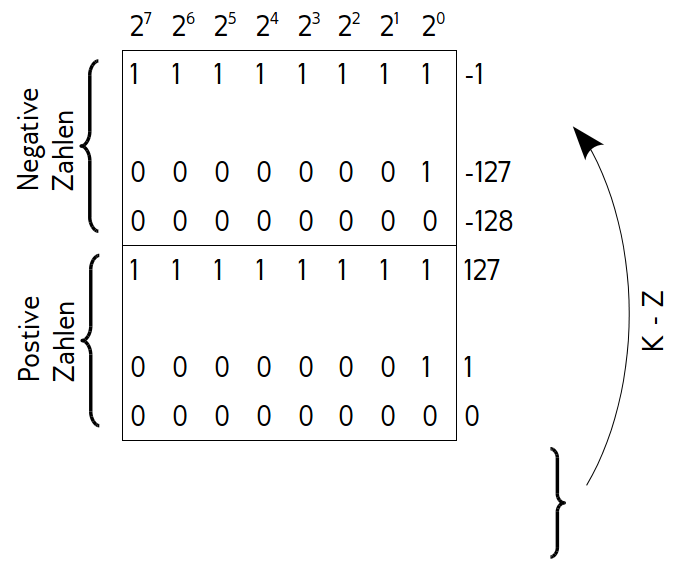
\includegraphics[width = 5.5cm, keepaspectratio]{images/tabelle_zweierkomplement.png}
  }
}
%
Die gängigste Form der Zahlensysteme sind Stellenwertsysteme. Eine Zahl $a$ wird in Form einer Reihe von Ziffern $z_i$ mit dazugehöriger Potenz der Basis $b^i$ dargestellt. Der Wert der Zahl ergibt sich dann als Summe der Werte aller Einzelstellen: $a = \sum\limits_{i}z_ib^i$.

\textbf{Umrechnung} in andere Zahlensysteme: Gegeben sei Zahl $Z$, umzuwandeln in System mit Basis $b$.
Eine angenehme Vorgehensweise gibt uns das \textbf{Horner Schema}\footnote{
Website mit Umrechnungen und Erklärungen: \url{http://www.arndt-bruenner.de/mathe/scripts/Zahlensysteme.htm}
}: Dividiere $Z$ durch $b$. Der Rest dieser Division ist die letzte Stelle der Zahl in der Basis $b$  (Einerstelle). Dividiere den Quotienten dieser Division wieder durch $b$. Der Rest dieser zweiten Division ergibt die zweite Stelle der Zahl in der neuen Basis. Wiederhole Divisionen, bis kein Rest mehr.


\section{Tabellen}
\subsection{Einfach}
\begin{center}
\begin{tabular}[c]{c | c | c || c| c | c || c | c || c | c | c || c| c| c}
\multicolumn{3}{c||}{Konjunktion}	&	\multicolumn{3}{c||}{Disjunktion} & \multicolumn{2}{c||}{Negation} & \multicolumn{3}{c||}{NAND} & \multicolumn{3}{c}{NOR}\\
\multicolumn{3}{c||}{UND}	&	\multicolumn{3}{c||}{ODER} & \multicolumn{2}{c||}{} & \multicolumn{3}{c||}{} & \multicolumn{3}{c}{}\\
\hline
$a$ & $b$ & $a$ $\wedge$ $b$ & $a$ & $b$ & $a$ $\vee$ $b$ & $a$ & $\bar{a}$ & $a$ & $b$ & $\overline{a \wedge b}$ & $a$ & $b$ & $\overline{a \vee b}$\\
\hline
0 & 0 & 0 & 0 & 0 & 0 & 0 & 1 & 0 & 0 & 1 & 0 & 0 & 1\\
0 & 1 & 0 & 0 & 1 & 1 & 1 & 0 & 0 & 1 & 1 & 0 & 1 & 0\\
1 & 0 & 0 & 1 & 0 & 1 & & & 1 & 0 & 1 & 1 & 0 & 0\\
1 & 1 & 1 & 1 & 1 & 1 & & & 1 & 1 & 0 & 1 & 1 & 0\\
\hline
\end{tabular}
\end{center}




%-----------------------------
\section{Zwei Bilder}

\begin{figure}[h!]
\centering
  \minipage{0.3\textwidth}
    \fbox{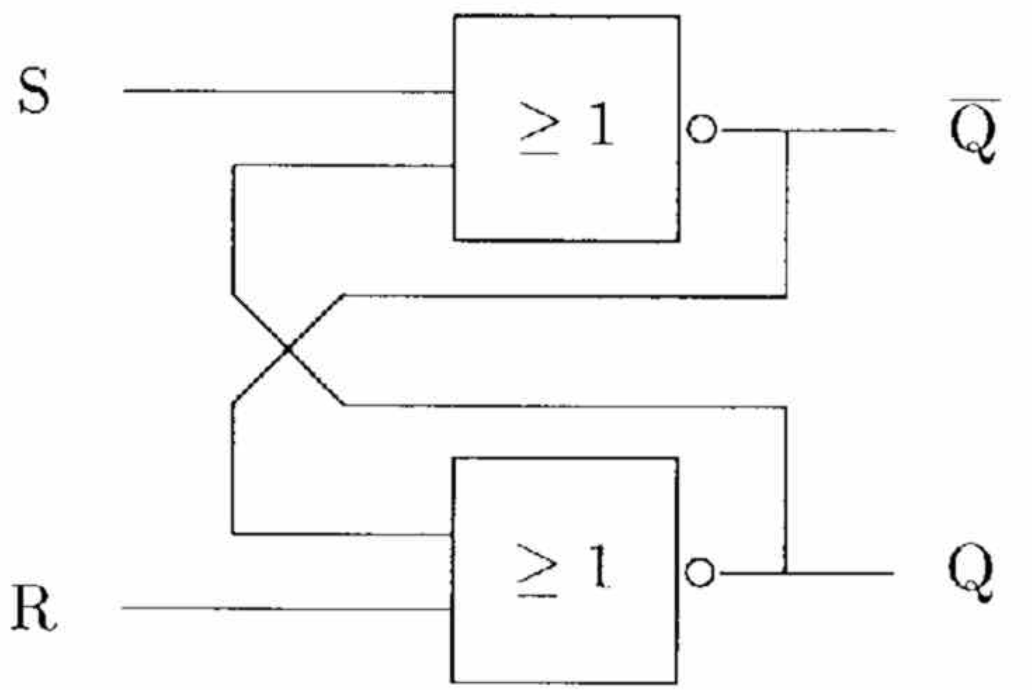
\includegraphics[height=2.5cm, keepaspectratio]{images/rsflipflop.png}}%
    \caption{RS-Flipflop}%
    \label{fig:rsflipflop}
  \endminipage\hspace{1cm}   
%
  \minipage{0.4\textwidth}
    \fbox{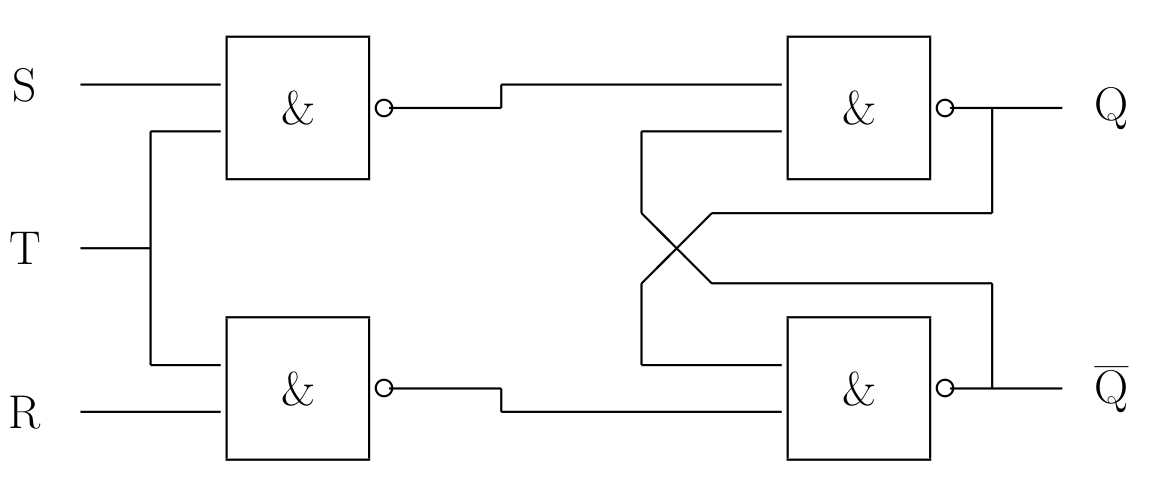
\includegraphics[height=2.5cm, keepaspectratio]{images/rsflipfloptakt.png}}%
    \caption{getaktetes RS-Flipflop}%
    \label{fig:rsflipfloptakt}
  \endminipage
\end{figure}

Dabei müssen wir eine Nebenbedingung $R \wedge S = 0$ setzen - $R$ und $S$ dürfen niemals gleichzeitig $= 1$ sein. In der Realisierung, dargestellt in Abb. \ref{fig:rsflipflop}, führt dies zu oszillationen. 

Will man ein taktgesteuertes RS-Flipflop, so braucht man lediglich das Taktsignal mit einem UND-Gatter jeweils mit dem $R$- und $S$-Eingang zu verbinden (siehe Abb. \ref{fig:rsflipfloptakt}).



\end{document}